\documentclass[tikz, border=5pt]{standalone}
\usepackage[utf8]{inputenc}
\usepackage{tikz}
\usetikzlibrary{arrows.meta} % Necesario para >=Stealth

\begin{document}
    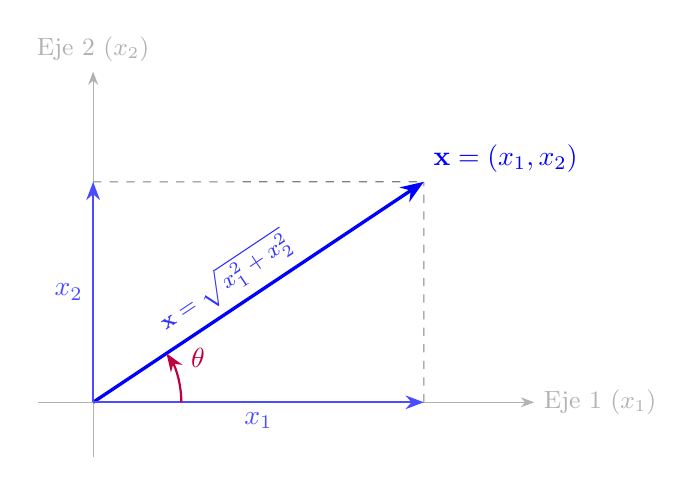
\begin{tikzpicture}[scale=1.4, >=Stealth]
        % Coordenadas
        \coordinate (O) at (0,0);
        \coordinate (X) at (3,2);
        \pgfmathsetmacro{\angle}{atan2(2,3)}
        
        % Ejes
        \draw[->, gray!60] (-0.5,0) -- (4,0) node[right] {\small Eje 1 ($x_1$)};
        \draw[->, gray!60] (0,-0.5) -- (0,3.0) node[above] {\small Eje 2 ($x_2$)};
        
        % Proyecciones
        \draw[dashed, gray] (3,0) -- (X);
        \draw[dashed, gray] (0,2) -- (X);
        
        % Vector
        \draw[->, very thick, blue] (O) -- (X);
        
        % Componentes
        \draw[->, thick, blue!70] (O) -- (3,0) node[midway, below] {$x_1$};
        \draw[->, thick, blue!70] (O) -- (0,2) node[midway, left] {$x_2$};
        
        % Ángulo
        \draw[purple, thick, ->] (O) ++(0:0.8) arc[start angle=0, end angle=\angle, radius=0.8];
        \node[purple, right] at (0.8, 0.4) {$\theta$};
        
        % Etiquetas
        \node[blue!80, rotate=\angle, anchor=south] at ({\angle}:1.6) {\footnotesize $\lVert \mathbf{x} \rVert= \sqrt{x_1^2+x_2^2}$};
        \node[blue] at (X) [above right] {$\mathbf{x}=(x_1,x_2)$};
    \end{tikzpicture}
\end{document}
